\documentclass{standalone}
\usepackage{tikz}
\usetikzlibrary{matrix}

\begin{document}

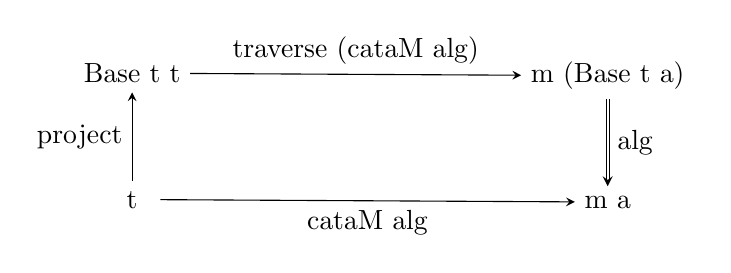
\begin{tikzpicture}
  \matrix (m) [matrix of math nodes,row sep=3em,column sep=12em,minimum width=2em]
  {
     \textrm{Base t t} & \textrm{m (Base t a)} \\
     \textrm{t}        & \textrm{m a} \\
  };
  \path[-stealth]
    (m-2-1) edge node [left]  {\textrm{project}} (m-1-1)
            edge node [below] {\textrm{cataM alg}} (m-2-2)

    (m-1-1) edge node [above] {\textrm{traverse (cataM alg)}} (m-1-2)

    (m-1-2) edge [double] node [right] {\textrm{alg}} (m-2-2);
\end{tikzpicture}

\end{document}
